\section{任务二}
给定如下明密文数据流，任务1中的三个转子和反射器的定义不变，但转子顺序不固定，请尝试恢复密钥K1和K2。（假设加密过程中，中速和慢速转子不转动）

明文WETTERVORHERSAGEHEUTE

密文EWGZDSATLWNEDBBCJUNGW

\subsection{思路分析}
\subsubsection{分割密钥空间}
实验给的明文和密文长度一样，且没有出现明文字母和密文字母相同的情况，因此可以认为这就是对应的明密文，即Crib，

由于加密的时候密钥K1和K2是合并起来的，穷举数量太大，因此需要分割密钥空间，我们可以类比2-DES的攻击，通过一些相同的中间量来脱去外层加密,把\(K_1\)和\(K_2\)分开

前面探讨过，\(|K_1| >> |K_2|\),所以我们寄希望于消除掉\(K_1\),先回复\(K_2\)

\subsubsection{寻找中间状态}
我们注意到这样的一种特殊的Crib，即内部能形成环路的Crib，因为接线板就是一个由连接线决定的单表代换，这个过程和K2没有关系，
enigma机的明文输入会经过一次接线板，而输出密文前也会经过一次接线板，这之间有一个中间状态。
我们就可以利用这个中间状态单独回复\(K_2\)，然后再去恢复\(K_1\)，实现对于密钥空间的分割，降低密钥恢复的复杂度。

以课程上的一个crib为例，
\begin{figure}[H]
    \centering
    
\includegraphics[width=0.8\textwidth]{figures/crib.png}
    \caption{Crib}
    \label{fig:Crib}
\end{figure}
明文里的W,经过接线板，\(K_1\)我们可以理解成一个可逆的单表带换，即\(K_1(W)=L_0\)，

然后密文的E，\(K_1(E)=L_1\)，此时我们发现明文的下一个也是E，它得到的中间状态也应该是\(L_1\),那这样我们就能消解掉接线板的影响

(值得注意的是，这里的Crib是一种交替的环路，就是从明文-密文-明文-密文...这样明密文交替进行的，这实际上会影响后续的数据结构，参考程序中并不是这样的，不过这又是后话了)
\subsubsection{建立关于\(K_2\)的方程}
我们利用这个中间状态来建立K2的方程：
它有一个\textbf{不随机现象}就是，\(L_0\)进\(L_0\)出，
而\(L_1\)本身就是\(L_0\)经过扰频器和反射器得到的，也就是说，知道\(L_0\)和\(K_2\),就能计算\(L_1,L_2\)
\[
L_{i-1} \xrightarrow{K_2} L_i
\]
我们简单把这个步骤记作\({Enc}_{K_2}\)
因此这中间的路径也被消解了，我们只需要关注首尾的\(L_0\),正确的K2应该能让\(L_0\)进\(L_0\)出

我们只需要遍历\(|K_2|\times|L_0|\)次，其中\(|L_0|=26\),这远远小于\(|K_1|\times|K_2|\)的穷举
当然这个也会有错误，但是我们多找几个环路，然后取交集，就能得到比较少的候选了。

其中对中间状态而言，正确的$K_2$必然满足$L_0$进且$L_0$出；对于错误的$K_2$，我们将环路看作随机置换，输入为$i,i \in \{A,B,\dots,Z\}$，输出为$\pi(i)$。满足环路即
$$
i = \pi(i)
$$
这里随机置换共$26!$种，结合错排数公式:
$$
D_n = n! \sum_{k=0}^n \frac{(-1)^k}{k!}
$$
得到错排率为
$$
Pr = \frac{D_{26}}{26!} = \sum_{k=0}^{26} \frac{(-1)^k}{k!} = 1 - 1 + \frac{1}{2!} -\frac{1}{3!}+...+\frac{1}{26!}
$$
利用$e^{-x}$的泰勒展开式：
$$
e^{-x} = \sum_{k=0}^{\infty}\frac{(-1)^k x^k}{k!}
$$
因此有$ Pr \approx e^{-1}  $。回到错误密钥但依然能形成环路的情况，即随机置换全部错排的对立面，对应概率为:
$$
Pr' = 1- Pr = 1- e^{-1} \approx 63.2\%
$$
可见错误率还是挺高的，需要结合后续其他条件筛掉错误密钥$K_2$。


当然这个也会有错误，但是我们多找几个环路，然后取交集，就能得到比较少的候选了
\subsubsection{根据环路恢复\(K_1\)以及\(K_2\)}
我们前面找到的可能的\(K_2\)的候选集，记为\(\{(L_0^{1i},K_2^1),(L_0^{2i},K_2^2),..., (L_0^{ni},K_2^n)\}\)
因为一个\(K_2\)可能对应多个\(L_0\),所以\(L_0^{1i},K_2^1\)可能有多个\(i\),即多个\(L_0\)对应同一个\(K_2\)
我们可以利用这些候选的\(K_2\)来恢复\(K_1\)，同时进一步筛选\(K_2\)
因为我们已知环路，比如W-E-E-T-T-W
那么就有\(K_1(W)=L_0\)，\(K_1(E)=L_1\)，\(K_1(T)=L_2\)，以此类推。
如何筛选呢？就是寻找矛盾，再回到完整的Crib，寻找\(K_1\)中已经有的字母，比如又找到一个W，它又会对应一个新的密文字母比如J

分两种情况
\begin{itemize}
    \item 如果J已经在\(K_1\)中出现过了，那么我们检查\({Enc}_{K_2}(K_1(W)) = K_1(J)\),如果不等，就排除这个\(K_1\),如果所有\(K_1\)都被排除，就排除这个\(K_2\)
    \item 如果J没有出现过，那么就可以继续扩展\(K_1(J) = {Enc}_{K_2}(K_1(W))\)
\end{itemize}
经过这轮筛选之后，我们就能恢复出\(K_1\)和\(K_2\)了
运行decrypt.py即可得到结果
\begin{figure}[H]
    \centering
    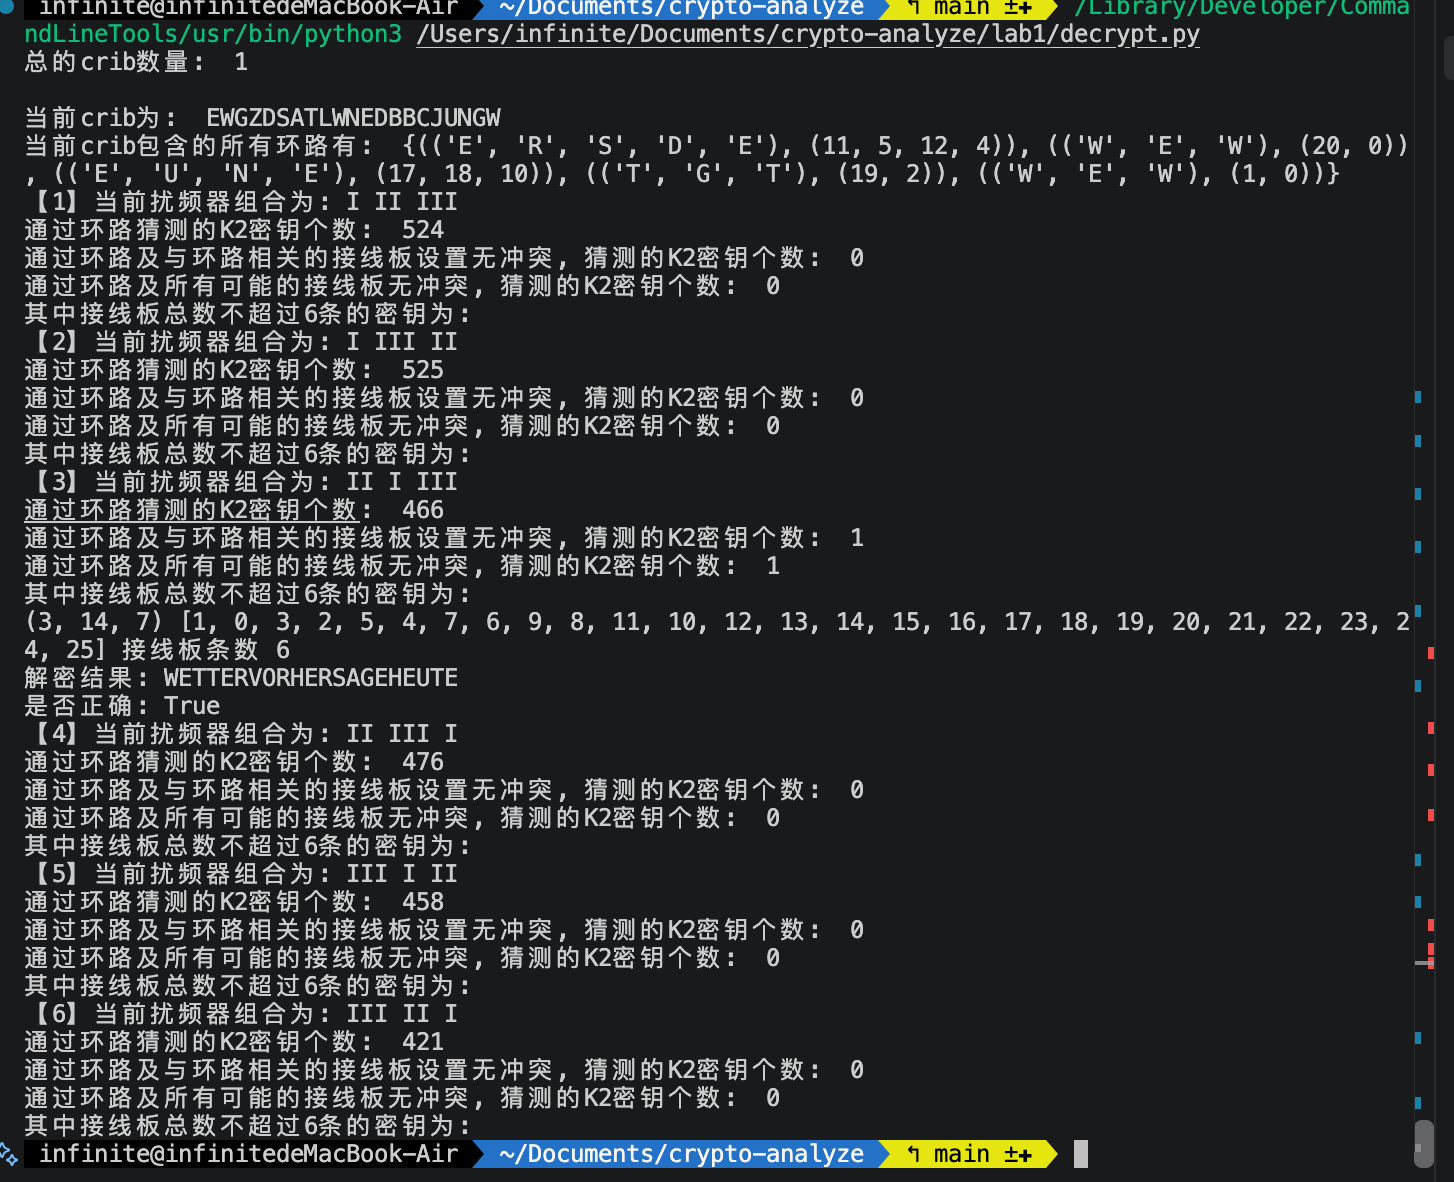
\includegraphics[width=0.8\textwidth]{figures/result3.png}
    \caption{result}
    \label{fig:res}
\end{figure}
最后\(K_1\)，\(K_2\)恢复的结果是：
\[
K_1=[1, 0, 3, 2, 5, 4, 7, 6, 9, 8, 11, 10, 12, 13, 14, 15, 16, 17, 18, 19, 20, 21, 22, 23, 24, 25]
\]

\[
K_2 = ((3, 14, 7),(II,I,III))
\]

